\section{An Introduction to Digital Electronics}
\label{lab_digital_electronics}

%\makelabheader %(Space for student name, etc., defined in master.tex)

\bigskip

\begin{enumerate}[wide]

\item A 74LS00 chip has four separate NAND gates on it.  (A pinout diagram is included in Appendix \ref{appendix_pinouts}.) To use this chip, you will need to connect pin 14 ($V_{CC}$) to $+5$ volts, and pin 7 to ground.  Use the logic switches (labeled S1, S2, etc.) on your proto boards as inputs into pins 1 and 2, and connect pin 3 to one of the logic indicator lights.  Does your chip produce the correct ``truth table'' for all four possible combinations of inputs?\label{part_verify_nand_gate}

\item Predict how you think your NAND chip would behave if one of the inputs were left unconnected.  Would it interpret the open input as a logical 0 or a logical 1?  Now do the experiment, disconnecting one of the inputs entirely, and toggling the other input between a 0 and 1 using a logic switch, as in part~\ref{part_verify_nand_gate}.  Was your prediction correct?  If not, rate your surprise and disappointment with the world on a scale from $-1$ to $-10$. \label{part_open_digital_inputs}

\item Suppose that you need an inverter (a ``NOT'' gate) for a circuit, but you happen not to have one in your kit.  Show how you can build your own inverter using a NAND gate.  Also show how you can build an OR gate out of two NOR gates.

\item Build a simple controller that might control a set of security lights outside a home.  The lights should go on when motion is detected nearby, but they should not come on during daytime hours.  The lights should also go on if the homeowner pushes a ``panic'' button.  If the lights come on due to motion outside, the homeowner should be able to turn them off by pushing a ``clear'' button.  There are four digital inputs: motion, daytime, panic, and clear.  Design and build a logic circuit with a single digital output that is high or low to control the lights based on these four inputs.  Connect the output of your circuit to one of the logic indicators on the right of your circuit boards.

\item Logic circuits can be used to do arithmetic on binary (base two) numbers.  Design and build a circuit that can add two 2-bit numbers.  Each of the inputs can be either 0, 1, 2, or 3, represented by two input bits as 00, 01, 10, or 11.  The output will be the binary representation from 0 to 6, using three output bits.  Test your circuit, using the logic switches on your board to control the inputs, and the logic indicators to view the outputs.  Keep good notes on how you build this circuit; you will use it again in a future lab.

\vspace{0.2in}
\begin{minipage}{.58\textwidth} %was .60

\item Sometimes you want to create a digital signal based on whether one voltage is larger than another.  For example, you may want an alarm to be switched from OFF to ON if some temperature, represented by a voltage, rises above some predetermined limit. The drawing to the right shows how to use an LM311 comparator to do this.  In the circuit below, if $V_+<V_-$, then pin 7 gets connected to pin 1 inside the chip, so that $V_{OUT}=0$.  Otherwise, $V_{OUT}=5$~volts.  Use your LM311 comparator to build a circuit whose output is 5 volts if an input voltage is less than 2.5 volts, and the output 0 volts if the input voltage is greater than 2.5 volts.  As a test input for your circuit, use a 1~kHz sine-wave from your function generator with an amplitude of 4 volts.
\end{minipage}
\begin{minipage}{.39\textwidth}

\hspace{0.25in}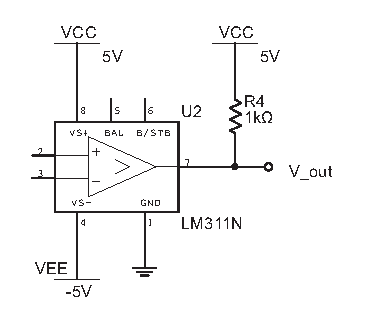
\includegraphics{digital_electronics/basic_lm311.eps}
\end{minipage}

\pagebreak[2]

\item What happens to your output when you increase the amplitude of your test input to 10 volts?  What determines the limitation on your input voltage?

\item If you look carefully at the output of your circuit in part 5 on a very fast time scale, you will see that each time the output switches, it actually makes multiple transitions, switching back and forth several times before settling down.  Why would it do this?  

\item To get only a single clean transition, you can make the modification of your circuit, shown below.  What is the voltage $V_+$ at the positive input if $V_{OUT}=0$ volts?  What is $V_+$ if $V_{OUT}=5$~volts?   Predict the values of the $V_+$ in each case, and test your prediction by measuring it with your friend, the oscilloscope.  How does the resistor $R_3$ prevent the multiple transitions you observed in the previous part?  (This clever little trick is called a ``Schmitt Trigger.'') \label{part_schmitt_trigger}

\begin{center}
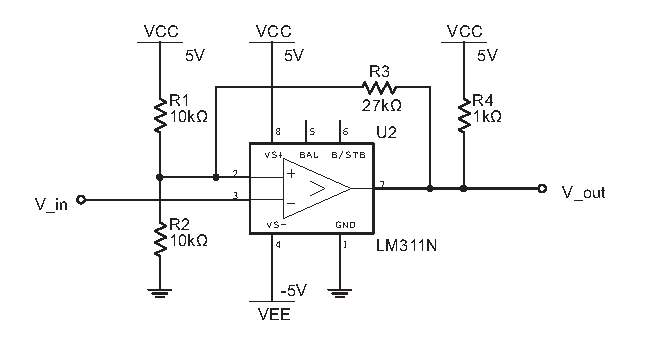
\includegraphics{digital_electronics/schmitt_trigger.eps}
\end{center}

%\item In the previous lab, you built a D/A converter.  Here, you will build a 2-bit A/D converter, to convert a variable input voltage of 0 to 3 volts to a set of two digital signals representing the numbers 00, 01, 10, and 11.  (0.00--0.99 volts gives digital 00; 1.00--1.99 volts gives digital 01, etc.)  The way it works is this: start by comparing the input signal to a 2 volt reference, and set the twos bit accordingly.  If $V_{IN}<2$, then compare it two a 1-volt reference, and set the ones bit.  If $V_{IN}>2$, then subtract off 2 volts from $V_{IN}$, and then set the ones bit by comparing $ V_{IN}-2$ volts to the 1-volt reference.  Build and test your circuit, and sketch another circuit showing how you would extend this idea to build a 4-bit A/D converter.

\end{enumerate}


\textbf{Possible Exam Questions:}

\begin{itemize}

\item Design a Schmitt trigger that gives a high output for $V_{IN}<1.1$ volts, and a low input for $V_{IN}>0.9$ volts.  Yes, you really have to remember how to build one of these from scratch!

\item Show how you can build an XOR gate using only OR and NAND gates.
\end{itemize}






